\documentclass[12pt,oneside]{article}
\usepackage[T1]{fontenc}
\usepackage[utf8]{inputenc}
\usepackage{lmodern}
\usepackage{amsmath,amssymb,amsthm,booktabs,graphicx,microtype}
\usepackage{tikz}
\usetikzlibrary{arrows.meta,positioning}
\newtheorem{proposition}{Proposition}
\newtheorem{corollary}[proposition]{Corollary}
\usepackage[margin=1in]{geometry}
\usepackage[colorlinks=true,linkcolor=blue,urlcolor=blue]{hyperref}
\hypersetup{pdftitle={Wash lending in vault networks: funding, incentives and loss transmission},
  pdfauthor={Sigma Labs}}
\frenchspacing
\newcommand{\pos}[1]{\left[#1\right]_+}
\title{Wash lending in vault networks:\\funding, incentives and loss transmission}
\author{Sigma Labs}
\date{9 September 2026}

\begin{document}
\maketitle
\begin{abstract}
A vault can finance borrowing against its own shares, allowing borrowers
to redeposit the proceeds and recover part of their interest payments
through share ownership. We study the resulting wash-lending loop in a
closed model with a fixed allocation between an external strategy and
a lending market. Consolidation shows that the loop can deploy idle
cash but cannot expand external investment beyond initial equity.
Borrowing redistributes the resulting income, with different incentives
for price-taking and strategic participants. We derive the funding
bound, the return decomposition and local liquidation thresholds, then
examine how losses in self-referential collateral can feed back into
vault value. The analysis distinguishes the priority of a secured loan
from the rights of passive vault holders, and market funding attribution
from verified circular borrowing. These distinctions provide a basis
for evaluating self-lending structures without treating gross balance
sheet growth, interest rebates and loss protection as equivalent.
\end{abstract}

\section{Introduction}
\label{sec:introduction}
Consider a vault that promises access to an external investment
strategy while retaining part of its assets in a lending market.
Suppose that market accepts the vault's own shares as collateral.
A holder can then borrow from the vault, deposit the proceeds back
into it, and pledge the newly issued shares. The vault grows, its
external investment can grow, and the borrower receives a larger share
of its income. Yet no new investor has supplied capital to the system.
What has the loop financed, and who bears the obligations it creates?

We call this arrangement \emph{wash lending}: borrowing funded by an
issuer or vault against claims on itself, with the proceeds returning
to the same balance sheet. The term describes a financing structure;
it does not by itself imply fictitious transactions or misconduct.
The economic issue is the overlap between the roles of borrower,
shareholder and lender. Interest paid by a borrower becomes vault
income, part of which returns to that borrower through its shares.
A contractual interest rate is therefore not enough to identify the
borrower's net payment to other participants.

\subsection{The question and the contribution}
The central question is how a loop can improve individual returns
without creating aggregate income from its internal payments. Our
answer starts with the use of cash. Under a fixed allocation rule,
redeposited borrowing directs a fraction of idle lending liquidity
into the external strategy. That additional deployment can generate
income. Interest then distributes the income between participants
according to their debt and share ownership. The distinction matters:
an increase in a holder's return can reflect additional external
investment, a transfer from another holder, or both.

The same accounting imposes a limit. If all borrowing is funded by
the vault, external investment cannot exceed the participants' initial
equity. A collateral rule allowing high leverage on an individual
position does not supply the cash required for that leverage across
the whole vault. Moreover, receiving an interest rebate does not
establish an incentive to borrow. A participant must compare leverage
with holding unlevered shares, which receive the same base vault yield.
A large holder also changes the rebate by changing its ownership share;
its decision differs from that of a price taker.

Risk introduces a further distinction. Borrower equity protects the
secured loan against a local collateral loss. It does not give passive
holders of the same vault share class priority in the vault's assets.
When those shares also secure loans on the vault's balance sheet, a
loss in external backing can affect both share value and loan recovery.
The paper develops these accounting and incentive results and uses
them to identify what a reported self-lending exposure can establish.
It does not estimate the probability of a run or claim that circular
funding alone determines its outcome.

\subsection{Approach, scope and relation to the literature}
We begin with a numerical example and then consolidate a closed
network consisting of a vault and its participants. All borrowing
proceeds are redeposited; the vault owns all lending claims; share
income is distributed pro rata; idle cash earns zero. The external
strategy's return and the allocation rule are specified rather than
derived from asset-market equilibrium. This deliberately narrow
setting makes the sources and recipients of income explicit.
We subsequently distinguish price-taking leverage choices from a
strategic borrower's choice, and use an exogenous collateral markdown
to separate liquidation from equity exhaustion. Opening the funding
perimeter to outside lenders is treated in an appendix.

The analysis relates to the financial-network perspective of Eisenberg
and Noe~\cite{eisenberg-noe}, where interdependent obligations must be
valued consistently with limited liability and debt priority. Our
self-referential NAV equation is a stylized valuation condition, not an
application of their clearing theorem: vault shares and their redemption
introduce claims whose settlement requires additional rules. It also
relates to the collateral-equilibrium literature reviewed by Fostel
and Geanakoplos~\cite{fostel-geanakoplos}, which studies feedback between
leverage and asset values. Here collateral limits are given, and the
focus is the funding and income feedback created when the lender holds
claims secured by its own shares.

Section~\ref{sec:example} follows the cash through a loop and a
redemption. Sections~\ref{sec:accounting} and~\ref{sec:returns} establish
what is conserved and how income is shared.
Section~\ref{sec:equilibrium} asks when those payments induce leverage;
Section~\ref{sec:loss} follows the obligations under stress.
Section~\ref{sec:case} turns the model into an interpretation of market
evidence. The epilogue returns to the design question raised by the
opening example: what does the loop enable while it is running, and
what must remain possible when a holder wants to leave?

\section{What wash lending changes: a motivating example}

\label{sec:example}
A vault $V$ accepts asset $S$ and issues shares $X$. It allocates half
its assets to an external strategy $L$ earning $s=8\%$, and half to a
market $\mathcal M$ lending $S$ against $X$ at $r=3\%$. The vault is
the sole lender and the participants below are its only shareholders.
Unborrowed cash earns zero. Rates are annualized simple income rates,
held constant for each comparison; the calculations are not compounded
APYs and exclude fees and losses.

Transactions occur before income accrues, with initial share NAV
normalized to $1S$. All shares minted by a looping borrower are also
pledged as collateral. The final position can be reached in successive
borrow, deposit and pledge steps, subject to liquidity and collateral
limits at every step. Figure~\ref{fig:flows} shows the flows between
the three parties.

\begin{figure}[htbp]
 \centering
 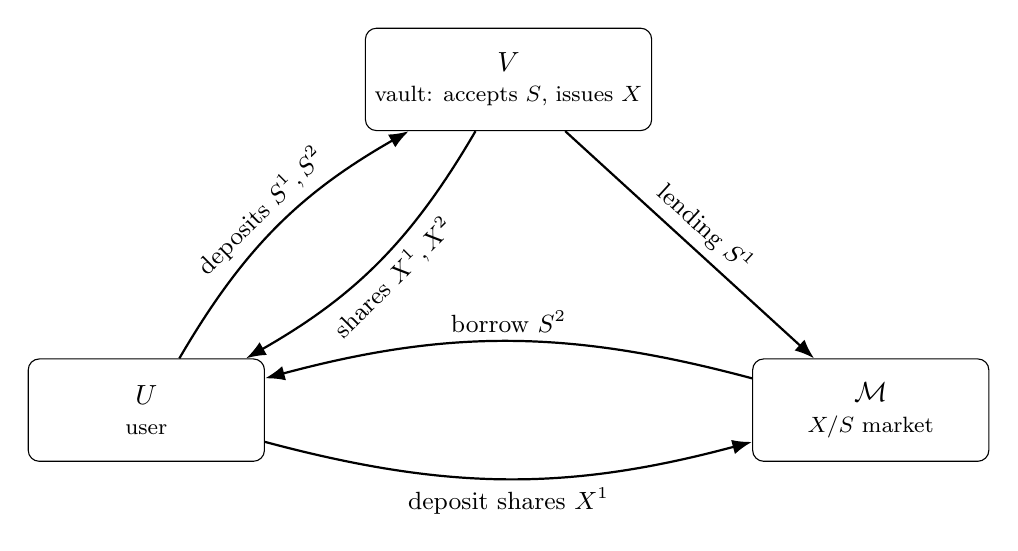
\begin{tikzpicture}[
   box/.style={draw,rounded corners,minimum width=3cm,minimum height=1.3cm,align=center},
   flow/.style={-{Latex[length=2.5mm]},thick},
   lab/.style={sloped,font=\small,inner sep=3pt}]
  \node[box] (V) at (0,4.2) {$V$\\[-1pt]\footnotesize vault: accepts $S$, issues $X$};
  \node[box] (U) at (-4.6,0) {$U$\\[-1pt]\footnotesize user};
  \node[box] (M) at (4.6,0) {$\mathcal M$\\[-1pt]\footnotesize $X/S$ market};
  \draw[flow] (U) to[bend left=15] node[lab,above] {deposits $S^1,S^2$} (V);
  \draw[flow] (V) to[bend left=15] node[lab,below] {shares $X^1,X^2$} (U);
  \draw[flow] (V) to node[lab,above] {lending $S^1$} (M);
  \draw[flow] (U) to[bend right=15] node[lab,below] {deposit shares $X^1$} (M);
  \draw[flow] (M) to[bend right=15] node[lab,above] {borrow $S^2$} (U);
 \end{tikzpicture}
 \caption{Flows in the motivating example. The user $U$ deposits $S^1$
 and $S^2$ into the vault $V$ and receives shares $X^1$ and $X^2$. The
 vault lends $S^1$ to the market $\mathcal M$; the user pledges $X^1$
 there and borrows $S^2$, which is redeposited in $V$.}
 \label{fig:flows}
\end{figure}

\subsection{Initial deposits}
$P_1$ and $P_2$ each deposit $100S$ and receive $100X$. The vault holds
$100S$ in $L$ and $100S$ idle in $\mathcal M$. Its annual income is
$100\times8\%=8S$, so each participant earns $4S$.

\subsection{Borrowing and redepositing}
$P_2$ pledges its shares, borrows $60S$, deposits the proceeds in $V$,
and pledges the additional $60X$. The resulting positions are
\[
 P_1=100X,\qquad P_2=160X-60S,\qquad T=260S.
\]
The vault has $130S$ in $L$ and a $130S$ lending position consisting
of $60S$ of loans plus $70S$ of cash. Its income and the participants'
net income are
\begin{align*}
 I_V &=130(0.08)+60(0.03)=12.2,\\
 I_1 &=\frac{100}{260}(12.2)\approx4.69,\\
 I_2 &=\frac{160}{260}(12.2)-1.8\approx5.71.
\end{align*}
The $1.8S$ interest payment is internal: $I_1+I_2=10.4S$, exactly
the income of $L$. Of its interest payment, $P_2$ recovers $160/260$;
the net payment to $P_1$ is $1.8(100/260)\approx0.692S$, equivalent
to a rate of $1.154\%$ on the $60S$ debt.

$P_2$'s debt/equity multiplier is $m=0.6$, while its lending-market
LTV is $60/160=37.5\%$. Using only the original $100X$ as pledged
collateral would instead give $60\%$ LTV; that is a different position.
The income gain comes from moving $30S$ of initially idle cash into
$L$. Allocating the initial $200S$ entirely to $L$ would have earned
$16S$, exceeding the loop's combined income, but would change the
vault's allocation and liquidity profile.

\subsection{Redemption changes ownership}
Suppose $P_1$ redeems $100X$ immediately, before income accrues.
Assume $L$ is redeemable at par: $V$ withdraws $50S$ from each venue,
leaving $80S$ in $L$ and $80S$ in $\mathcal M$, of which $60S$ is
lent. $P_2$ still has $160X-60S$ and now owns all vault shares. Its
net income becomes
\[
 I_2=80(0.08)+60(0.03)-60(0.03)=6.4S.
\]
It recovers all interest paid to the vault. LTV is unchanged, but
market utilization rises from $60/130$ to $60/80$. An actual rate
model could therefore change the quoted borrow rate. Complete rebate
does not make pledged shares freely redeemable or make loans liquid.

The example separates the benefit of deploying cash from the benefit
of receiving interest paid by someone else. It also reveals their
liquidity cost: the external strategy holds more assets and the lending
market retains less cash. To determine how far this process can go,
we next consolidate the balance sheets.

\section{How the loop works: accounting and funding}
\label{sec:accounting}
\subsection{Participants, claims and the consolidation boundary}
Let $e_i>0$ be participant $i$'s initial equity, $y_i=m_i e_i$ its debt,
and $h_i=e_i+y_i$ its share value at the initial NAV. Include passive
holders as $m_i=0$. Write
\[
 E=\sum_i e_i,\qquad Y=\sum_i y_i,\qquad T=E+Y,\qquad
 \varphi=\frac{Y}{T}.
\]
The vault allocates fraction $0<\varepsilon<1$ to $L$, with return
$s\geq0$, and $1-\varepsilon$ to $\mathcal M$, at borrow rate
$r\geq0$. All market debt is
owed by these participants, all proceeds are redeposited, and the vault
owns all lending claims. These closure assumptions are needed for the
identities below. At a later NAV $q$, a deposit of $dS$ mints $d/q$
shares; nominal share counts must not be confused with asset values.

The vault's assets are
\[
 \underbrace{\varepsilon T}_{L}
 +\underbrace{Y}_{\text{loans}}
 +\underbrace{C}_{\text{idle cash}}=T,
 \qquad C=(1-\varepsilon)T-Y=E-\varepsilon T.
\]
Pledged $X$ is security for the loans, not an additional vault asset.
Consolidating the vault and its shareholders cancels the internal loan
and share claims and leaves $\varepsilon T+C=E$ of external assets.

\subsection{The funding bound}
\begin{proposition}[Funding and external investment]
\label{prop:funding}
Under the closed-network assumptions above, every feasible position
satisfies
\begin{equation}
 Y\leq(1-\varepsilon)(E+Y)
 \quad\Longleftrightarrow\quad
 \frac{Y}{E}\leq\frac{1-\varepsilon}{\varepsilon}.
 \label{eq:funding}
\end{equation}
External investment obeys $\varepsilon T\leq E$, with equality at full
market utilization. For $s\geq0$, external income is at most $sE$.
\end{proposition}
\begin{proof}
The outstanding loans cannot exceed the vault's lending allocation:
$Y\leq(1-\varepsilon)T$. Substituting $T=E+Y$ yields
\eqref{eq:funding}. Equivalently, idle cash
$C=E-\varepsilon T$ must be nonnegative. At full utilization $C=0$,
so $\varepsilon T=E$. Multiplication by $s\geq0$ gives the income
bound.
\end{proof}
Define utilization
\[
 u=\frac{Y}{(1-\varepsilon)(E+Y)},\qquad
 \varphi=(1-\varepsilon)u.
\]
Full utilization fixes $Y=(1-\varepsilon)E/\varepsilon$ and
$\varepsilon T=E$. Thus looping can deploy all initial equity into
$L$, but cannot increase the external allocation beyond $E$ in this
closed model. Combined income is at most $sE$. Individual profits can
still differ because interest redistributes that income.

\subsection{Collateral capacity and redemption capacity}
Funding and collateral are separate constraints. With liquidation LTV
$\ell_i$, a recursive position must satisfy
\[
 \frac{m_i}{1+m_i}\leq\ell_i,
 \qquad m_i\leq\frac{\ell_i}{1-\ell_i}.
\]
A practical maximum $M_i$ can be lower to allow a liquidation buffer.
A feasible terminal balance sheet does not itself prove that a
particular transaction sequence has enough liquidity to reach it.

A redemption of $wS$ that preserves the allocation fractions requires
$(1-\varepsilon)w\leq C$ if debt remains outstanding. It also requires
$\varepsilon w$ to be withdrawable from $L$. Without that allocation
constraint, liquid $L$ assets may fund more redemptions, but the vault's
portfolio then changes.

The funding bound settles what the loop can invest. It leaves open
who benefits from that investment, since a loan is an asset of the
vault and a liability of a participant who also owns vault shares.
The next step is to follow both sides of each interest payment.

\section{How the loop pays: income and ownership}
\label{sec:returns}
\subsection{Conservation and distribution of income}
\begin{proposition}[Return decomposition]
\label{prop:returns}
Vault income is $I_V=\varepsilon sT+rY$. The return per unit of vault
shares and participant $i$'s net return on equity are
\begin{align}
 c_v&=\varepsilon s+r\varphi,\\
 A_i&=(1+m_i)c_v-rm_i
     =c_v+m_i\Delta_v,\qquad
 \Delta_v=\varepsilon s-r(1-\varphi).
 \label{eq:return}
\end{align}
Consequently,
\begin{equation}
 \sum_i e_i A_i=\varepsilon sT.
 \label{eq:conservation}
\end{equation}
\end{proposition}
\begin{proof}
Participant $i$ receives $h_iI_V/T$ and pays $ry_i$. Dividing the
difference by $e_i$ gives~\eqref{eq:return}. Summing net income over
participants cancels the $rY$ paid to and received from the vault,
leaving~\eqref{eq:conservation}.
\end{proof}
A passive holder earns $c_v$, including borrow-market income. It does
not earn only $\varepsilon s$.

\subsection{A borrower's own payment and marginal carry}
Participant $i$ owns fraction $\alpha_i=h_i/T$ of the shares. Of its
own payment $ry_i$, it recovers $\alpha_i ry_i$, so the net payment
to other holders is $(1-\alpha_i)ry_i$. It also receives
$\alpha_i r(Y-y_i)$ from other borrowers. Hence
\[
 e_iA_i=\varepsilon s h_i
       -r(1-\alpha_i)y_i+\alpha_i r(Y-y_i).
\]
For a sole borrower with passive equity $x_1$ and own equity $x_2$,
this reduces to
\[
 T=x_1+x_2+y,\qquad b_{\mathrm{eff}}=r\frac{x_1}{T},\qquad
 I_2=\varepsilon s(x_2+y)-b_{\mathrm{eff}}y.
\]
Relative to no loop, its gain is
$y(\varepsilon s-rx_1/T)$; the passive holder gains $rx_1y/T$.
A concentrated borrower can therefore benefit even when the quoted
rate exceeds $s$, subject to funding and collateral feasibility.

By contrast, $r(1-\varphi)$ in~\eqref{eq:return} is the financing term
in the \emph{price-taking incremental carry}. It is not generally the
net rate on a particular borrower's own interest bill. The ownership
share $\alpha_i$ and the aggregate debt fraction $\varphi$ are distinct.

The distinction between an ownership rebate and incremental carry
is the bridge from accounting to behavior. The payment identity holds
for any feasible position. To predict a position, however, we must
specify what the participant can change and which quantities it takes
as given.

\section{From the rebate to leverage choice}
\label{sec:equilibrium}
\subsection{The price-taking benchmark}
A participant treating $r$ and $\varphi$ as fixed chooses
$m_i\in[0,M_i]$ to maximize~\eqref{eq:return}. The best response is
\[
 m_i\in
 \begin{cases}
 \{M_i\},&\Delta_v>0,\\
 [0,M_i],&\Delta_v=0,\\
 \{0\},&\Delta_v<0.
 \end{cases}
\]
If $a_i$ is an outside-option return, participation additionally requires
\[
 \max\{c_v,\ c_v+M_i\Delta_v\}\geq a_i.
\]
The test $A_i(M_i)\geq a_i$ alone is insufficient: when
$\Delta_v<0$, holding unlevered shares pays more than borrowing. If
participants withdraw equity to take their outside option, $E$ must
also be determined in equilibrium. Holding $E$ fixed instead describes
a population whose equity remains in the vault.

At fixed $Y$, a participant with $m_i<Y/E$ receives net interest:
\[
 \left.\frac{\partial A_i}{\partial r}\right|_{Y,m_i}
 =\frac{Y-m_iE}{E+Y}>0.
\]
This is a wealth-transfer effect. It does not imply upward-sloping
optimal borrowing demand: at the same fixed aggregate state,
$\partial\Delta_v/\partial r=-(1-\varphi)<0$.
A higher rate can make share ownership more attractive while making
additional leverage less attractive.

\subsection{Closing the model with supply and rates}
For a specified utilization-based rate rule $r=r(u)$, fixed equity,
and no participation exit, the benchmark equilibrium solves
\[
 Y=\sum_i e_i m_i,\qquad
 u=\frac{Y}{(1-\varepsilon)(E+Y)},\qquad
 m_i\in\operatorname{BR}_i(r(u),\varphi),\qquad 0\leq u\leq1.
\]
This is the endogenous-supply formulation. Imposing an unrelated fixed
supply $\bar S$ and $Y=\bar S$ would conflict with the vault allocation
unless $\bar S=(1-\varepsilon)E/\varepsilon$, or the allocation rule
were explicitly changed.

At fixed $r$, more aggregate debt raises each fixed-$m_i$ return:
\[
 \left.\frac{\partial A_i}{\partial Y}\right|_{r,m_i}
 =(1+m_i)r\frac{E}{(E+Y)^2}\geq0.
\]
But with a differentiable equilibrium rate schedule $r(Y)$,
\begin{align*}
 \frac{d\Delta_v}{dY}
 &=\frac{E}{(E+Y)^2}\bigl[r(Y)-(E+Y)r'(Y)\bigr],\\
 \frac{dA_i}{dY}
 &=(1+m_i)r\frac{E}{(E+Y)^2}
   +\bigl[(1+m_i)\varphi-m_i\bigr]r'(Y),
\end{align*}
where $m_i$ is held fixed. Rising utilization can offset the rebate.
Multiple equilibria require a demonstrated fixed-point structure;
they do not follow from the rebate identity alone.

\begin{corollary}[A limit to price-taking carry]
\label{cor:carry}
For $r\geq0$, a feasible closed-network position satisfies
\[
 \Delta_v\leq\varepsilon(s-r).
\]
Consequently $r\geq s$ rules out strictly positive price-taking carry.
\end{corollary}
\begin{proof}
Equation~\eqref{eq:funding} implies $1-\varphi=E/T\geq\varepsilon$.
Substitute this inequality into
$\Delta_v=\varepsilon s-r(1-\varphi)$.
\end{proof}
This result links the behavioral calculation back to the funding
bound. A rebate cannot be increased independently of the cash needed
to finance it. The conclusion concerns incremental leverage at a given
aggregate state; a strategic borrower's finite change in ownership
requires a different comparison.

\subsection{The strategic borrower}
A large borrower changes its ownership share and the rebate by looping.
Hold all initial equities and the other borrowers' debt $Y_{-i}$ fixed,
and let $y$ be borrower $i$'s choice. With
$T=E+Y_{-i}+y$ and $H_{-i}=E-e_i+Y_{-i}$, its income is
\[
 R_i(y)=\varepsilon s(e_i+y)
       +r\left[\frac{(e_i+y)(Y_{-i}+y)}{T}-y\right].
\]
At a fixed quoted rate,
\[
 R_i'(y)=\varepsilon s-\frac{rEH_{-i}}{T^2},\qquad
 R_i''(y)=\frac{2rEH_{-i}}{T^3}\geq0.
\]
The objective is convex, rather than linear. On a feasible interval a
maximum occurs at an endpoint, but the decision must compare total
income at those endpoints; the atomistic carry test is not its rule.
If the borrower also moves $r(Y)$, the first derivative gains the term
\[
 r'(Y)\left[(e_i+y)\varphi-y\right],
\]
and convexity need not survive. Entry or exit can lower interest costs
and reduce rebates simultaneously, so their combined effect has no
universal sign.

A return calculation can therefore explain why a loop is chosen without
establishing that it can be unwound. The remaining question concerns
the claims themselves: what happens when the collateral behind a loan
is also a claim on the lender's assets?

\section{When the loop is stressed: losses and recovery}
\label{sec:loss}
\subsection{The local secured-loan calculation}
Consider a position with equity $e$, collateral $(1+m)e$, and debt
$me$, all valued in the loan asset. Let collateral fall by fraction
$\delta\in[0,1]$, holding debt fixed. Without intervening liquidation,
remaining borrower equity, borrower loss and lender shortfall are
\begin{align*}
 Q(\delta)&=e\pos{1-(1+m)\delta},\\
 L_J(\delta)&=e\min\{(1+m)\delta,1\},\\
 L_D(\delta)&=e\pos{(1+m)\delta-1}.
\end{align*}
They satisfy $L_J+L_D=\delta(1+m)e$. The lender shortfall begins
\emph{after} the borrower has lost its equity; it must not be charged
against that equity a second time.

For $m>0$, the liquidation trigger and equity-wipeout threshold are
\begin{equation}
 \boxed{\delta_{\mathrm{liq}}=1-\frac{m}{\ell(1+m)},\qquad
        \delta_A=\frac{1}{1+m}.}
 \label{eq:thresholds}
\end{equation}
An initially healthy position has $\delta_{\mathrm{liq}}\geq0$.
At the maximum multiplier $m=\ell/(1-\ell)$ it has no initial
liquidation buffer. For $0<\ell<1$, liquidation is triggered before
equity wipeout.

\begin{center}
\begin{tabular}{rrrr}
\toprule
$m$ & $\ell$ & $\delta_{\mathrm{liq}}$ & $\delta_A$\\
\midrule
4 & 0.830 & 3.61\% & 20.00\%\\
6 & 0.915 & 6.32\% & 14.29\%\\
15 & 0.945 & 0.79\% & 6.25\%\\
\bottomrule
\end{tabular}
\end{center}
These are illustrative parameters, not claims about current markets.
Liquidation incentives, slippage, oracle delays and incomplete execution
change actual recoveries. For example, if liquidation of all collateral
repays only a fraction $\eta\leq1$ of its marked value, the residual
shortfall is $\pos{me-\eta(1-\delta)(1+m)e}$; this is a recovery
scenario, not the no-liquidation equity calculation above. Morpho's
published bad-debt description explicitly distinguishes the LLTV trigger
from collateral exhaustion after the liquidation
incentive~\cite{morpho}.

With heterogeneous positions and separate collateral accounts,
aggregate lender shortfall under the same exogenous shock is
\[
 L_D^{\mathrm{agg}}(\delta)
 =\sum_{i:m_i>0}e_i\pos{(1+m_i)\delta-1}.
\]
The first positive shortfall appears just above
$\min_{i:m_i>0}1/(1+m_i)$. One borrower's unused equity does not
protect another borrower's lender unless there is an explicit pooled
guarantee. There is no additional test equating summed shortfalls to
all borrowers' initial equity.

\begin{figure}[htbp]
 \centering
 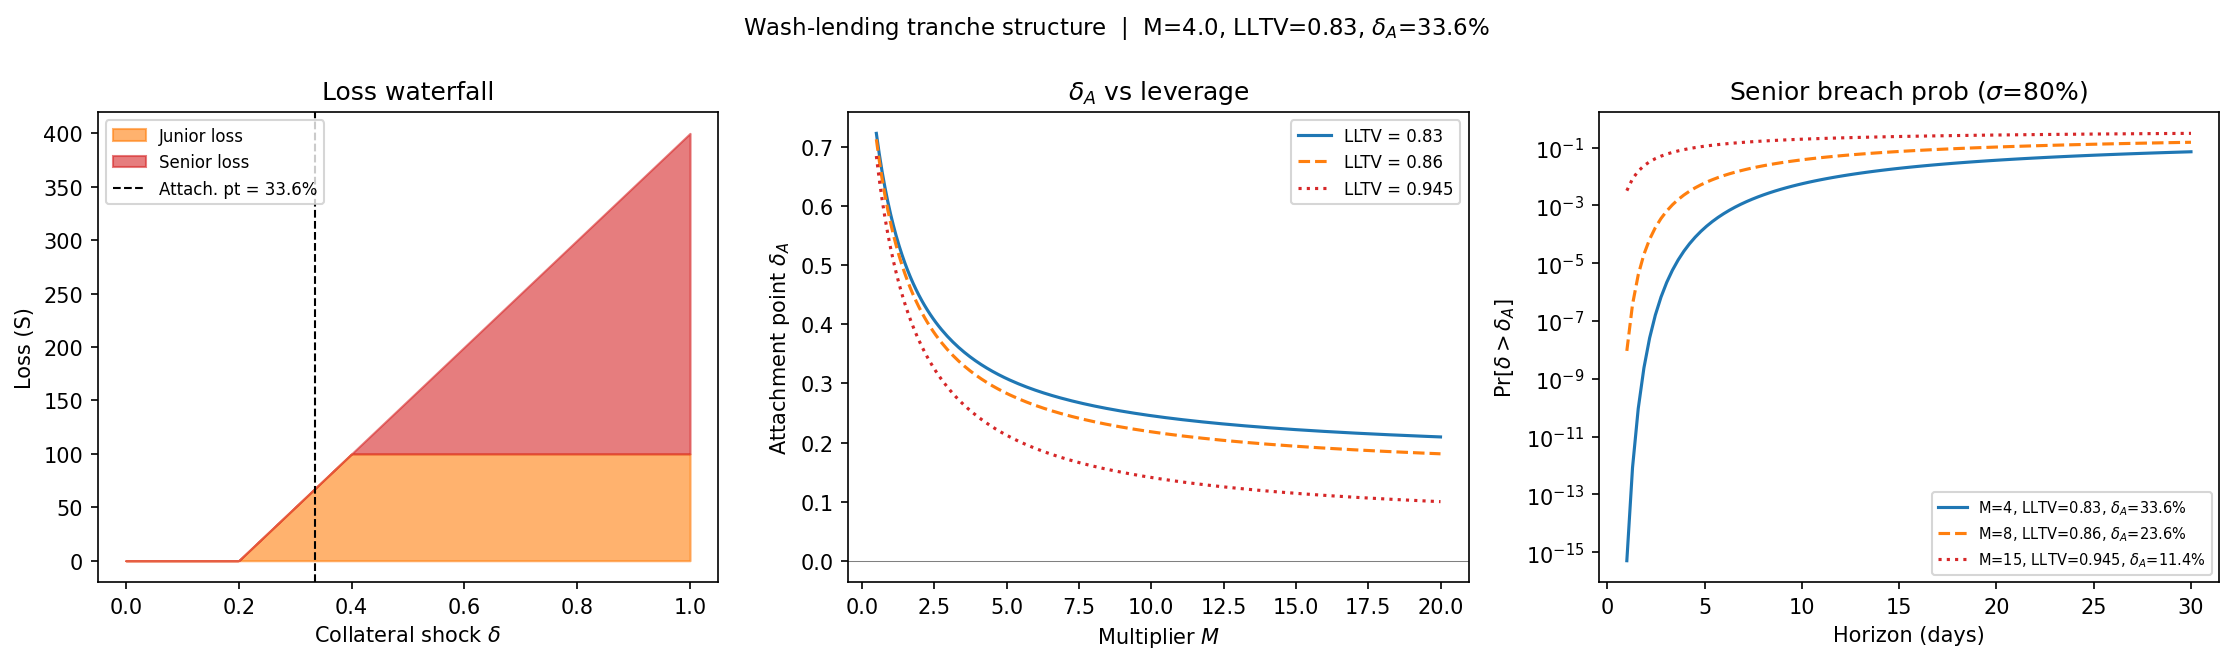
\includegraphics[width=\linewidth]{wash_tranche.png}
 \caption{Local secured-loan losses and thresholds, generated by
 \texttt{wash\_tranche.py}. The loss calculation assumes an exogenous
 collateral markdown, fixed debt and no intervening liquidation. The
 liquidation line is a reference trigger. Curves are restricted to
 initially feasible leverage. These are not a consolidated vault-loss
 waterfall or a calibrated default forecast.}
 \label{fig:thresholds}
\end{figure}

\subsection{Debt priority and the common share class}
The loan claim has priority over the borrower's residual collateral
value. But passive and looping holders own the same vault share class
in this model. Passive holders have no contractual priority over
looping holders in redeeming $V$, and a loss in $L$ reduces the value
of every share immediately. Loan losses recognized by the vault also
reduce the common NAV. The secured loan has a junior equity buffer;
the whole vault is not thereby a CDO with passive holders as seniors.

This matters because the collateral is itself a claim on the lender.
If $B$ is the post-shock value of the vault's external assets including
cash, $q$ its share NAV, and $n_i$ borrower $i$'s pledged share count,
a stylized simultaneous mark is
\[
 qT=B+\sum_i\min\{y_i,qn_i\},
\]
where initial outstanding shares are $T$, and liquidation costs and
share burns are omitted. If all loans remain recoverable, $B$ falling
by $\lambda$ lowers NAV by $\lambda/T$ at once. If $qn_i<y_i$,
loan write-downs feed back into NAV. Recoverability depends on who can
buy or redeem seized shares and with what external liquidity. The
formula is a consistency condition under its marking assumptions,
not an execution or settlement model. It shows why one cannot add
pledged share values to vault assets as independent backing.

\subsection{Price risk and the time to exit}
For ETH-denominated loans against ETH-denominated vault shares, the
relevant collateral return is the share/ETH basis. At the initial
mark, $(1+m)e-me=e$ leaves net ETH exposure on equity, but leverage
still amplifies losses in that basis. Small observed day-to-day
volatility does not establish safety against slashing, contract loss
or a discontinuous discount on redemption.

If a zero-drift arithmetic return were Gaussian with annualized
volatility $\sigma$, its terminal loss probability at horizon $\tau$
would be
\[
 \Pr(\delta_\tau>\delta_A)
 =\Phi\left(-\frac{\delta_A}{\sigma\sqrt\tau}\right).
\]
This is not the probability of crossing the threshold at any time
before $\tau$. Under a driftless Brownian model that first-passage
probability is $2\Phi(-\delta_A/(\sigma\sqrt\tau))$ for a positive
constant barrier. Neither expression captures jumps, endogenous NAV
feedback or failed liquidations. There is no probabilistic claim in
Figure~\ref{fig:thresholds}.

Stress analysis should distinguish oracle detection, liquidation
execution, collateral sale or redemption, and lender withdrawal. The
exit horizon depends on available cash, repayment flows and competing
redemptions. It cannot be inferred from collateral volatility alone.
Different shocks enter this sequence at different points. A fall in
external income reduces carry; a loss of backing reduces NAV; issuance
without corresponding assets dilutes claims; a withdrawal restriction
changes the set of feasible exits. Under the price-taking assumptions,
$\varepsilon s=0$ and $r>0$ imply negative incremental carry. That
income statement alone determines neither the speed of deleveraging
nor the associated capital loss.

This distinction sets the boundary of the model's risk conclusions.
Local leverage identifies a collateral buffer. Ownership identifies
who receives income and shares recognized losses. Settlement and
redemption rules determine whether collateral value can become cash
in time. A market application must supply all of these inputs.

\section{From the model to market evidence}
\label{sec:case}
The closed model is useful because every payment has an identified
recipient and every loan has an identified source. Public market
snapshots often provide a different object: outstanding borrowing
against an issuer's tokens and the issuer's share of lending supply.
To use that evidence, we must distinguish a funding attribution from
the closed loop defined in Section~\ref{sec:introduction}.

\subsection{What a funding attribution measures}
For lender share $\alpha_k$ of market $k$ and gross debt $B_k$ against
the relevant collateral, its pro-rata attribution is
\[
 F=\sum_k\alpha_k B_k.
\]
Unlike $\varphi=Y/T$, $\alpha_k$ is a \emph{share of market supply}.
It is neither a borrower's share of vault income nor the fraction of
vault backing financed through loops.

Appendix~\ref{app:snapshot} retains an attributed historical snapshot
as an illustration of this calculation. Its reported funding and
backing amounts produce a ratio near $30\%$. The role of the example
is methodological: neither that ratio nor the accounting model provides
a verified estimate of an issuer's circular borrowing without evidence
about the use of loan proceeds.

\subsection{Tracing funds, income and claims}
A loan against an issuer's token need not finance a redeposit into that
issuer. Proceeds may fund another asset or leave the system. Establishing
$T=E+Y$ for this case therefore requires tracing borrowing proceeds,
mints, redemptions and the relevant consolidation perimeter. Pro-rata
funding attribution alone does not establish that identity or quantify
TVL double counting.

The income mapping also requires care. USDe, sUSDe and maturity-specific
principal tokens are not interchangeable pro-rata claims on all reserve
income. Ethena documents discretionary reward distributions into sUSDe and states
that deposited USDe is not itself lent out by the staking contract. Its
reserve-fund and reward mechanics also prevent a direct identification
of negative protocol income with negative staking
rewards~\cite{ethena}.
A case-specific model must identify which legal or contractual entity
lends reserves, who receives that interest, and how it reaches each
collateral token. The remaining backing cannot simply be assumed to
be invested in a single basis strategy.

Even $\alpha_k=100\%$ means only that the attributed lender supplies
all liquidity in that market. A borrower does not recover all interest
unless it also receives all the corresponding distributed income.
Market lender concentration alone does not determine leverage,
liquidation order, or the size of the borrower's rebate.

\subsection{Observable implications and limits}
The useful follow-up to a snapshot is to measure the flow of borrowed
funds, income pass-through, actual leverage and LLTV by position,
oracle and redemption rules, and stressed exit liquidity. Those inputs
connect a funding attribution to a model of returns and losses.

The model suggests concrete accounting checks. Where the closed-network
assumptions hold, shareholder income net of borrowing costs must equal
external strategy income. At fixed initial equity and allocation, additional redeposited
debt must reduce idle cash by $\varepsilon$ per unit borrowed. A rise
in lending-market utilization without a corresponding change in the
measured debt fraction would signal that the assumed funding perimeter
or allocation has changed. These checks test the mapping of a system
to the model before any behavioral or risk interpretation is attempted.

The behavioral claims require additional evidence. An estimated response
of borrowing to rates must distinguish changes in the outside option,
income distribution, ownership concentration and loan supply. Observed
positive net interest income for a low-leverage holder is not evidence
that higher rates caused that holder to borrow more. Likewise, testing
loss transmission requires realized recovery prices and redemption
flows, rather than collateral marks alone.

The present analysis holds the external strategy, loan denomination and
allocation rule fixed. Fees, rewards paid from outside the modeled
system, asset-price effects, heterogeneous claim classes and strategic
withdrawals can change the conclusions. A dynamic extension would need
to specify the timing of interest accrual, NAV updates, margin calls and
cash settlement. The identities derived here provide consistency
conditions for that extension, not a substitute for it.

\section{Epilogue: what remains when the loop unwinds}
\label{sec:epilogue}
Return to the initial vault. A holder borrows $60S$, redeposits it,
and increases the external investment by $30S$. Both participants
receive more income than before the loop. The improvement is real
within the model: previously idle cash has been put to work. The
interest paid along the way determines how that income is shared.
Consolidation makes the source of the improvement visible without
erasing the obligations that make it possible.

Those obligations matter when the passive holder leaves. Its exit
changes the ownership of the interest stream, consumes cash and raises
utilization even though the remaining borrower's LTV is unchanged.
The remaining holder may recover every interest payment and still
face a binding constraint on redemption. The ability to receive the
income on a claim is different from the ability to turn that claim
into the asset needed to repay a loan.

For a vault designer, this gives a practical interpretation of the
funding bound. An allocation to lending is also a reserve of potential
withdrawal liquidity, to the extent that it remains unborrowed.
Looping can convert that cash into external investment, while changing
who depends on future repayments or liquidations. Evaluating the
conversion requires the external strategy's return and liquidity,
the distribution of debt and ownership, and the path by which a
position can close. A generous collateral limit cannot answer those
questions on its own.

For an observer, the same reasoning changes how a self-lending headline
should be read. A large gross position may contain substantial internal
claims; a small measured funding share may coexist with concentrated
ownership or a narrow liquidation buffer. Funding attribution is a
starting point for tracing dependencies. Its economic meaning emerges
only after the income and recovery rights are attached to the relevant
participants.

Wash lending therefore deserves analysis at both the transaction and
the consolidated levels. The transaction view reveals incentives,
priority and cash requirements. The consolidated view identifies the
external assets that ultimately support the claims. Keeping those
views consistent explains the loop's productive use of idle cash,
limits the returns that can be attributed to it, and locates the
questions that remain when the loop must unwind.

\clearpage
\appendix
\section{External lenders and ordinary leveraged carry}
\label{app:external}
When an independent lender finances the loop and the vault does not
receive the borrowing interest, a collateral yield $s_V$ gives return
\[
 A=s_V+m(s_V-r).
\]
Ignoring fees, a lender with utilization $u$ earns $ur$. If its
outside option is $s_0$ and the borrower's alternative is unlevered
vault shares, the joint improvement window is
\[
 \frac{s_0}{u}<r<s_V.
\]
There is no requirement that lender yield be below the borrower's
carry spread. The window is nonempty exactly when $us_V>s_0$.
For an illustrative parameter choice, $s_V=3.75\%$, $s_0=1.46\%$, $u=80\%$ give a window from
$1.825\%$ to $3.75\%$. The corresponding borrower returns are
\begin{center}
\begin{tabular}{rrr}
\toprule
$m$ & $r=2.12\%$ & $r=3.00\%$\\
\midrule
5 & 11.90\% & 7.50\%\\
10 & 20.05\% & 11.25\%\\
15 & 28.20\% & 15.00\%\\
\bottomrule
\end{tabular}
\end{center}
These are gross simple rates before risk, costs and compounding effects.
Common denomination removes a mechanical exchange-rate mismatch at the
initial mark; it does not eliminate basis, liquidity or liquidation risk.

If outside lenders instead share the same market as $V$, let $\alpha$
be the fraction of loan interest received by $V$, and let
$T=E+Y$ still hold because all borrowing is redeposited. Then
\[
 c_v=\varepsilon s+\alpha r\frac{Y}{T},\qquad
 \sum_i e_iA_i=\varepsilon sT-(1-\alpha)rY.
\]
The payment to outside lenders no longer cancels within the vault-holder
perimeter. Market supply and the vault's own allocation must also be
accounted for separately.

\section{TVL conventions and the financing limit}
\label{app:tvl}
For equity $e$ and multiplier $m$, collateral is $(1+m)e$ and debt is
$me$. A collateral-only gross TVL convention reports $(1+m)e$; one
that adds the drawn lender claim reports $(1+2m)e$. If all supplied
liquidity is counted, including idle cash, it instead reports
$(1+m)e+S_{\mathcal M}$, where $S_{\mathcal M}$ is total market supply.
None of these is net equity, which remains $e$ for the borrower.

For $m=15$, these first two gross measures are $16e$ and $31e$.
A collateral limit of $\ell=0.945$ allows at most
$m=\ell/(1-\ell)\approx17.18$, but it does not provide the required
loan liquidity. In the closed wash-lending system,
\eqref{eq:funding} separately bounds the equity-weighted average
multiplier. If every holder used $m=15$, the vault would need
$\varepsilon\leq1/16$; a half-external allocation cannot fund that
aggregate position. Gross balance-sheet amplification must therefore
be reported together with the source of funds and the consolidation
boundary.

\section{An attributed market snapshot}
\label{app:snapshot}
This appendix preserves a market-level estimate attributed to
\texttt{@yieldsandmore} on 20 May 2026, concerning Ethena-backed
lending against USDe-related collateral~\cite{yam}. The source thread
was not independently retrievable at preparation of this paper.
The transcribed figures are used solely to illustrate the funding
attribution in Section~\ref{sec:case}; they are not a verified dataset,
current balances or evidence that the closed-network assumptions hold.

All amounts in USD millions. The attribution and verification status are
described above.
\begin{center}
\small
\begin{tabular}{llrrrr}
\hline
\textbf{Venue} & \textbf{Market} & \textbf{Ethena} & \textbf{USDe+sUSDe}
  & \textbf{Lender} & \textbf{Est.\ self-} \\
               &                 & \textbf{supplied} & \textbf{borrowed}
  & \textbf{share}  & \textbf{lending} \\
\hline
Aave    & Plasma USDT0    & 368.0 & 556.0 & 47.4\%  & 263.3 \\
Aave    & Mantle USDT0    & 168.0 &  58.1 & 100.0\% &  58.1 \\
Aave    & Ethereum USDtb  & 140.0 &  46.7 & 82.5\%  &  38.5 \\
Aave    & MegaETH USDm    & 550.0 & 398.9 & 91.2\%  & 363.8 \\
Morpho  & Base Prime USDC & 252.9 &   0.0 & 54.3\%  &   0.0 \\
Morpho  & Ethereum USDtb  & 105.0 & 105.3 & 99.7\%  & 105.0 \\
Kamino  & Sentora USDG    & 250.0 & 250.0 & 100.0\% & 250.0 \\
Juplend & Bitwise USDG    & 251.0 & 251.0 & 100.0\% & 251.0 \\
\hline
\textbf{Total} & & \textbf{2084.9} & \textbf{1666.0} & & \textbf{1329.7} \\
\hline
\end{tabular}
\end{center}

Using the displayed rows, attributed funding totals $1329.7$ million
and gross debt totals $1666.0$ million. The gap is $336.3$ million of
debt attributed to other lenders. Products of the rounded supply shares
and debt amounts need not reproduce every displayed attribution exactly.
With the reported backing denominator of $4.4$ billion, $F/T$ is about
$30.2\%$; gross collateralized debt divided by backing is about $37.9\%$.
These are different measures, not lower and upper bounds on a verified
closed-loop debt ratio.

\subsection{A conditional numerical illustration}
If the closed model did apply, illustrative assumptions
$\varepsilon=0.53$, $s=9\%$, $r=6\%$ and $\varphi=0.30$ would give
\[
 c_v=6.57\%,\qquad \Delta_v=0.57\%,\qquad
 A(m=6)=9.99\%.
\]
Here $u=0.30/0.47\approx63.8\%$, so the aggregate funding constraint
holds. Aggregate debt/equity is only $\varphi/(1-\varphi)\approx0.429$.
If all active loopers use $m=6$ and all other holders are passive, active
looper equity must be $Y/6$, or about $7.14\%$ of total initial equity.
Calling $m=6$ representative of every holder would be inconsistent.
At $\ell=0.915$, that local position begins liquidation after a
$6.32\%$ collateral decline and loses all initial equity at $14.29\%$
without prior liquidation. These assumptions do not estimate Ethena's
actual carry or a loss threshold for its passive holders.


\clearpage
\begin{thebibliography}{9}
\bibitem{eisenberg-noe}
Larry Eisenberg and Thomas H. Noe (2001).
\emph{Systemic Risk in Financial Systems}.
Management Science, 47(2), 236--249.
\href{https://doi.org/10.1287/mnsc.47.2.236.9835}{doi:10.1287/mnsc.47.2.236.9835}.

\bibitem{fostel-geanakoplos}
Ana Fostel and John Geanakoplos (2013).
\emph{Reviewing the Leverage Cycle}.
Cowles Foundation Discussion Paper No.\ 1918.
\href{https://cowles.yale.edu/node/139539}{Cowles Foundation publication record}.

\bibitem{morpho}
Morpho. \emph{Managing Bad Debt: How-to Guide}.
Protocol documentation, accessed 9 September 2026.
\href{https://docs.morpho.org/curate/tutorials-v1/bad-debt/}{Morpho documentation}.

\bibitem{ethena}
Ethena. \emph{Rewards Mechanism}.
Protocol documentation, accessed 9 September 2026.
\href{https://docs.ethena.fi/protocol-overview/rewards-mechanism}{Ethena documentation}.

\bibitem{yam}
\texttt{@yieldsandmore} (attributed, 20 May 2026).
Thread on Ethena self-lending exposure.
\href{https://x.com/yieldsandmore/status/2057150511883710628}{Original thread link}.
Verification status and use are stated in Appendix~\ref{app:snapshot}.
\end{thebibliography}

\end{document}
